% **************************************************
% Document Class Definition
% **************************************************
\documentclass[%
paper=A4,                    % paper size --> A4 is default in Germany
twoside=false,                % onesite or twoside printing
openright,                    % doublepage cleaning ends up right side
parskip=full,                % spacing value / method for paragraphs
chapterprefix=true,            % prefix for chapter marks
11pt,                        % font size
headings=normal,            % size of headings
bibliography=totoc,            % include bib in toc
listof=totoc,                % include listof entries in toc
titlepage=on,                % own page for each title page
captions=tableabove,        % display table captions above the float env
draft=false,                % value for draft version
]{scrreprt}%

% **************************************************
% Debug LaTeX Information
% **************************************************
%\listfiles

% **************************************************
% Information and Commands for Reuse
% **************************************************
\newcommand{\thesisTitle}{Xây dựng chatbox sử dụng Machine Learning}
\newcommand{\thesisName}{Phạm Hùng Vỹ - 15521037 \\ Lê Nhựt Vinh - 15521016}
\newcommand{\thesisSubject}{Báo cáo}
\newcommand{\thesisDate}{13/06/2019}
\newcommand{\thesisVersion}{1.0}

\newcommand{\teacher}{Huỳnh Tuấn Anh}
\newcommand{\thesisFirstReviewer}{Jane Doe}
\newcommand{\thesisFirstReviewerUniversity}{\protect{Clean Thesis Style University}}
\newcommand{\thesisFirstReviewerDepartment}{Department of Clean Thesis Style}

\newcommand{\thesisSecondReviewer}{John Doe}
\newcommand{\thesisSecondReviewerUniversity}{\protect{Clean Thesis Style University}}
\newcommand{\thesisSecondReviewerDepartment}{Department of Clean Thesis Style}

\newcommand{\thesisFirstSupervisor}{Jane Doe}
\newcommand{\thesisSecondSupervisor}{John Smith}

\newcommand{\thesisMainUniversity}{\protect{Đại học quốc gia Thành phố Hồ Chí Minh}}
\newcommand{\thesisUniversity}{\protect{Trường Đại học Công nghệ thông tin}}
\newcommand{\thesisUniversityDepartment}{Khoa công nghệ phần mềm}
\newcommand{\thesisUniversityInstitute}{Institut for Clean Thesis Dev}

\newcommand{\figureBigSize}{10cm}
\newcommand{\figureMediumSize}{10cm}
% **************************************************
% Load and Configure Packages
% **************************************************
\usepackage[utf8]{inputenc}        % defines file's character encoding
\usepackage[english]{babel} % babel system, adjust the language of the content
\usepackage[                    % clean thesis style
figuresep=colon,%
sansserif=false,%
hangfigurecaption=false,%
hangsection=true,%
hangsubsection=true,%
colorize=full,%
colortheme=bluemagenta,%
bibsys=bibtex,%
bibfile=bib-refs,%
bibstyle=alphabetic,%
]{cleanthesis}

\hypersetup{                    % setup the hyperref-package options
pdftitle={\thesisTitle},    % 	- title (PDF meta)
pdfsubject={\thesisSubject},% 	- subject (PDF meta)
pdfauthor={\thesisName},    % 	- author (PDF meta)
plainpages=false,            % 	-
colorlinks=false,            % 	- colorize links?
pdfborder={0 0 0},            % 	-
breaklinks=true,            % 	- allow line break inside links
bookmarksnumbered=true,        %
bookmarksopen=true            %
}

% Overwrite clean thesis formating
\usepackage[T1]{fontenc}
\usepackage[sfdefault]{AlegreyaSans} %% Option 'black' gives heavier bold face
%% The 'sfdefault' option to make the base font sans serif
\renewcommand*\oldstylenums[1]{{\AlegreyaSansOsF #1}}
\usepackage[justification=centering]{caption}

% **************************************************
% Document CONTENT
% **************************************************
\begin{document}

    % --------------------------
    % rename document parts
    % --------------------------
    %\renewcaptionname{ngerman}{\figurename}{Abb.}
    %\renewcaptionname{ngerman}{\tablename}{Tab.}
    \renewcaptionname{english}{\figurename}{Fig.}
    \renewcaptionname{english}{\tablename}{Tab.}

    % --------------------------
    % Front matter
    % --------------------------
    \pagenumbering{roman}            % roman page numbing (invisible for empty page style)
    \pagestyle{empty}                % no header or footers
    % !TEX root = ../chatbot-report.tex
%
% ------------------------------------  --> cover title page
\begin{titlepage}
	\pdfbookmark[0]{Cover}{Cover}
	\flushright
	\centering{
		\uppercase{ \LARGE \thesisMainUniversity} \\[6mm]
		\uppercase{ \LARGE \thesisUniversity} \\[4mm]
		\uppercase{ \LARGE \thesisUniversityDepartment} \\[4mm]
%		
\includegraphics[width=6cm]{gfx/Clean-Thesis-Logo} \\[2mm]
	}
	\hfill
	\vfill
	{\LARGE \color{ctcolortitle}\textbf{\thesisTitle} \\[10mm]}
	\rule[5pt]{\textwidth}{.4pt} \par
	\begin{minipage}[t]{.27\textwidth}
		\raggedleft
		\textit{Giảng viên hướng dẫn}
	\end{minipage}
	\hspace*{15pt}
	\begin{minipage}[t]{.65\textwidth}
		{\Large\teacher} \par
	\end{minipage} \\[5mm]
	\begin{minipage}[t]{.27\textwidth}
		\raggedleft
		\textit{Sinh viên thực hiện}
	\end{minipage}
	\hspace*{15pt}
	\begin{minipage}[t]{.65\textwidth}
		{\Large\thesisName}
	\end{minipage} \\[10mm]
	\vfill
	\vfill
	\textit{\large\thesisDate} \\
	Version: \thesisVersion
\end{titlepage}

        % INCLUDE: all titlepages
    \cleardoublepage

    \pagestyle{plain}                % display just page numbers
    %
    % !TEX root = ../chatbot-report.tex
%
\pdfbookmark[0]{Lời cảm ơn}{Thank}
\chapter*{Lời cảm ơn}
\label{sec:thank}
\vspace*{-10mm}

Nhóm chúng em hoàn thành được tốt đồ án môn học này, không thể không nói đến công lao của thầy
\teacher. Chúng em xin chân thành cảm ơn thầy đã tận tâm hướng dẫn chúng em. Bên cạnh đó, nhóm
cũng xin gửi lời cảm ơn chân thành đến các anh chị khóa trên, các bạn trong và ngoài lớp đã sẵn lòng chia sẻ tài liệu
cũng như kinh nghiệm từng trải của bản thân để nhóm chúng em học tập và tránh mắc những sai lầm, tiết kiệm được thời
gian trong quá trình thực hiện đồ án.

Tuy nhiên, do kiến thức và khả năng của chúng em còn nhiều hạn chế, do đó không tránh khỏi những thiếu sót, yếu kém.
Chúng em rất mong nhận được những ý kiến đóng góp quý báu của thầy cô và các bạn học cùng lớp để đồ án được hoàn
thiện hơn và rút ra được kinh nghiệm.
Sau cùng, chúng em xin kính chúc quý thầy cô ở Khoa Công nghệ Phần mềm, đặc biệt là thầy \teacher thật dồi dào sức khỏe để
tiếp tục thực hiện sứ mệnh cao đẹp của mình là truyền đạt kiến thức cho thế hệ mai sau.
Nhóm xin chân thành cảm ơn!
 % INCLUDE: acknowledgement
    \cleardoublepage
    %
    \setcounter{tocdepth}{2}        % define depth of toc
    \tableofcontents                % display table of contents
    \cleardoublepage

    % --------------------------
    % Body matter
    % --------------------------
    \pagenumbering{arabic}            % arabic page numbering
    \setcounter{page}{1}            % set page counter
    \pagestyle{maincontentstyle}    % fancy header and footer

    % !TEX root = ../chatbot-report.tex
%
\chapter{Tổng quan}
\label{sec:intro}

\section{Giới thiệu}
Dự đoán giá cổ phiếu là việc mà các nhà kinh tế thường xuyên bị hỏi.
Tuy nhiên việc dự đoán chính xác là một việc khó có thể làm vì có rất nhiều yếu tố ảnh hưởng.
Như cổ phiếu của một công ty chịu rất nhiều ảnh hưởng từ hoạt động công ty, chính phủ, quyết định của các nhà đầu tư.
Một số cá nhân, tổ chức có ảnh hưởng cực kì lớn tới giá cổ phiếu.
Với sự phát triển của internet thì thông tin được lan truyền rất nhanh, thông tin dường như gây ảnh hưởng đến giá cổ phiếu ngay lập tức

Đối với vàng thì thực sự không có một cá nhân tổ chức nào có thể nắm được quyền lực cụ thể.
Có rất nhiều nhân tố, một dòng twitter của tổng thống Mỹ Donald Trump không thể nào có những ảnh hưởng đáng kể tới giá vàng như việc tuyên bố cấm cửa Huawei của ông.

Thời trước đã có nhiều phương pháp để dự đoán giá vàng bằng phương pháp xây dựng mô hình thuần thống kê như
\begin{itemize}
    \item Autoregressive (AR)
    \item Moving Average (MA).
    \item Autoregressive Moving Average (ARMA)
    \item Autoregressive Integrated Moving Average (ARIMA)
    \item Seasonal Autoregressive Integrated Moving Average (SARIMA)
\end{itemize}
Những phương pháp này yêu cầu người dùng cần có rất nhiều kiến thức để tinh chỉnh tham số, đưa ra các dự đoán

Ngày nay, với sự phát triển của Machine Learning, có nhiều thuật toán mới tiến bộ, không yêu cầu người dùng phải
có kiến thực rộng lớn như cây quyết định, học sâu.

Trong cây quyết định có thuật toán nổi tiếng như XGBoost, LGB. Những thuật toán yêu cầu người dùng có khả năng đưa ra nhiều feature nhất có thể
để có thể đưa ra dự đoán chính xác

Học sâu có các mạng dòng họ Recurrent Neural Networks thường được sử dụng vì khả năng ghi nhớ thông tin trước đó. Phổ biến nhất là LSTM, GRU. Những thuật toán
này không cần người dùng đưa ra những feature nhưng những mạng này thường yêu cầu dữ liệu rất nhiệu và sức mạnh tính toán rất lớn để đưa ra dự đoán chính xác.

Gần đây, Facebook có đưa ra thuật toán Prophet. Sử dụng các tham số mặc định, Prophet đưa ra các dự đoán chính xác đánh ngạc nhiên mà không
tốn nhiều tài nguyên để tính toán.

 % INCLUDE: introduction






 % INCLUDE: introduction
    % !TEX root = ../chatbot-report.tex
%
\chapter{Dữ liệu}
\label{sec:data}

\section{Dữ liệu}
Được lấy từ package python fix\_yahoo\_finance. Gói này lấy thông tin từ trang Yahoo Finance và chuyển thành Panda Dataframe.
Bảng này gồm 7 cột:
\begin{itemize}
    \item Date: ngày
    \item Open: giá lúc mở phiên
    \item Close: giá lúc đóng phiên
    \item High: giá cao nhất trong ngày
    \item Low: giá thấp nhất trong ngày
    \item Adj close: giá đóng phiên
    \item Volume: số lượng bán ra
\end{itemize}

Dự liệu được lấy từ thị trướng chứng khoán, chính vì vậy, có những ngày nghỉ như ngày lễ, ngày thứ 7, chủ nhật sẽ không có dữ liệu.
Ngoài ra dữ liệu không theo quy luật năm, có tính mùa, có quy luật trong tuần. Trong các năm, hầu như giá vào mùa xuân sẽ cao hơn cái ngày còn lại

\section{Mạng học sâu}
Tiền xử lý dữ liệu
\begin{itemize}
    \item Đối với những ngày không có dữ liệu thì điền dữ liệu bằng ngày trước để có tính liên tục \\
    \item Giữ lại cột: Date, Close. Đổi tên cột Date thành ds, Close thành y. Bỏ các cột còn lại(Theo quy chuẩn) \\
    \item Chuẩn hoá dữ liệu cột y bằng MinMaxScalar với khoảng (0, 1) \\
    \item Giữ 90 ngày cuối để xác minh. Những ngaỳ còn lại để đem train \\
    \item Dữ liệu đầu vào: sẽ ra giá của ngày hiện tại + 89 ngày trước \\
    Dữ liệu đầu ra là giá vàng 90 ngày sau ngày hôm nay. Vậy sẽ bỏ qua 89 ngày đầu của bộ dữ liệu (thiếu dữ liệu ngày trước đó) \\
\end{itemize}
\textbf{Model}
    LSTM là Recurrency network có khả năng quyết định quên, ghi nhớ và xuất trạng thái \\
    Mạng ban đầu gồm 5 lớp: LSTM -> Dropout -> LSTM -> Dropout -> Dense \\


    Mạng lúc sau là : LSTM -> Dense \\
    Đầu vào có dạng (batch\_size, 90, 1) \\
    Đầu ra có dạng (90) (dự đoán 90 ngày cùng lúc) \\
    Mạng được train với loss function là MAE \(MAE = \frac{1}{n}\sum_{i=1}^{n}|f_i - p_i|\), optimizer là Adam \\
\textbf{Kết quả}
    Sử dụng MAE đánh giá, chỉ số có giá trị càng nhỏ thì càng chính xác. Sau ta khi inverse transform ta đc \\
    Mạng ban đầu 5 lớp là 6. \\
    Mạng sau là 4.2 \\

\section{Prophet}
Tiền xử lý dữ liệu
\begin{itemize}
    \item Đối với những ngày không có dữ liệu thì điền dữ liệu bằng ngày trước để có tính liên tục \\
    \item Giữ lại cột: Date, Close. Đổi tên cột Date thành ds, Close thành y. Bỏ các cột còn lại(Theo quy chuẩn) \\
    \item Tới đây thôi nha prophet không yêu cầu tiền xử lý gì hết \\
\end{itemize}
\textbf{Model}
Prophet với tham số mặc định, không sử dụng seasonal, weekly, holiday \\
\textbf{Kết quả}
Sử dụng MAE đánh giá. MAE = 0.99 (WTF ??)
 % INCLUDE: data work
    % !TEX root = ../chatbot-report.tex
%
\chapter{Tiền xử lý dữ liệu}
\label{sec:preprocessing}

\cleanchapterquote{Innovation distinguishes between a leader and a follower.}{Steve Jobs}{(CEO Apple Inc.)}

\Blindtext[2][1]

\section{System Section 1}
\label{sec:system:sec1}

\Blindtext[1][2]

\begin{figure}[htb]
	
\includegraphics[width=\textwidth]{gfx/Clean-Thesis-Figure}
	\caption{Figure example: \textit{(a)} example part one, \textit{(c)} example part two; \textit{(c)} example part three}
	\label{fig:system:example1}
\end{figure}

\Blindtext[1][2]

\section{System Section 2}
\label{sec:system:sec2}

\Blindtext[1][2]

\begin{figure}[htb]
	
\includegraphics[width=\textwidth]{gfx/Clean-Thesis-Figure}
	\caption{Another Figure example: \textit{(a)} example part one, \textit{(c)} example part two; \textit{(c)} example part three}
	\label{fig:system:example2}
\end{figure}

\Blindtext[2][2]

\section{System Section 3}
\label{sec:system:sec3}

\Blindtext[4][2]

\section{Conclusion}
\label{sec:system:conclusion}

\Blindtext[2][1]
    % INCLUDE: system
    % !TEX root = ../chatbot-report.tex
%
\chapter{Model}
\label{sec:model}

\section{LSTM}
\label{sec:model:LSTM}
\textbf{Recurrent neural network} \\[0.2em]
Con người không bắt đầu suy nghĩ từ đầu mỗi giây.
Khi bạn đọc bài luận này, bạn hiểu từng từ dựa trên sự hiểu biết của bạn về các từ trước đó.
Bạn không nên ném mọi thứ đi và bắt đầu suy nghĩ lại từ đầu. Suy nghĩ của bạn
có sự lưu lại.

Mạng lưới thần kinh truyền thống có thể làm được điều này, và nó có vẻ như là một
thiếu sót lớn.
Ví dụ, hãy tưởng tượng bạn muốn phân loại loại sự kiện nào đang diễn ra tại mọi thời điểm trong phim.
Nó không rõ làm thế nào một mạng lưới thần kinh truyền thống có thể sử dụng lý lẽ của nó về các sự kiện trước đó trong phim để thông báo cho những sự kiện sau này.

Recurrent neural network giải quyết vấn đề này. Chúng là các mạng có các vòng lặp trong đó, cho phép thông tin tồn tại.
\begin{figure}[!htb]
    \center{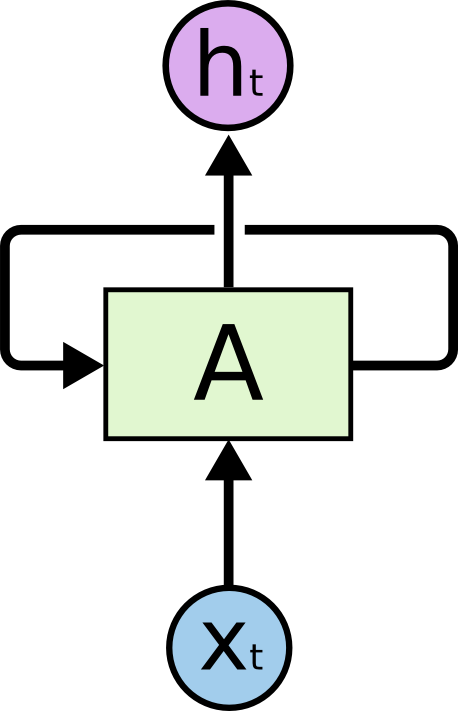
\includegraphics[width=2cm]
    {figure/model/RNN-rolled.png}}
    \caption{\label{fig:rnn-rolled} Recurrent Neural Network có vòng lặp.}
\end{figure}

Trong sơ đồ trên, một đoạn của mạng thần kinh, \(A\), xem xét một số xt đầu vào và xuất ra một giá trị
\(h_t\).Một vòng lặp cho phép thông tin được truyền từ một bước của mạng sang bước tiếp theo.

Những vòng lặp này làm cho Recurrent neural network có vẻ như bí ẩn.
Tuy nhiên, nếu bạn suy nghĩ nhiều hơn một chút, hóa ra họ không phải là một mạng lưới thần kinh bình thường.
Recurrent neural network có thể được coi là nhiều bản sao của cùng một mạng, mỗi bản tin truyền cho một người kế nhiệm.
Xem xét những gì xảy ra nếu chúng ta bỏ vòng lặp:

\begin{figure}[!htb]
    \center{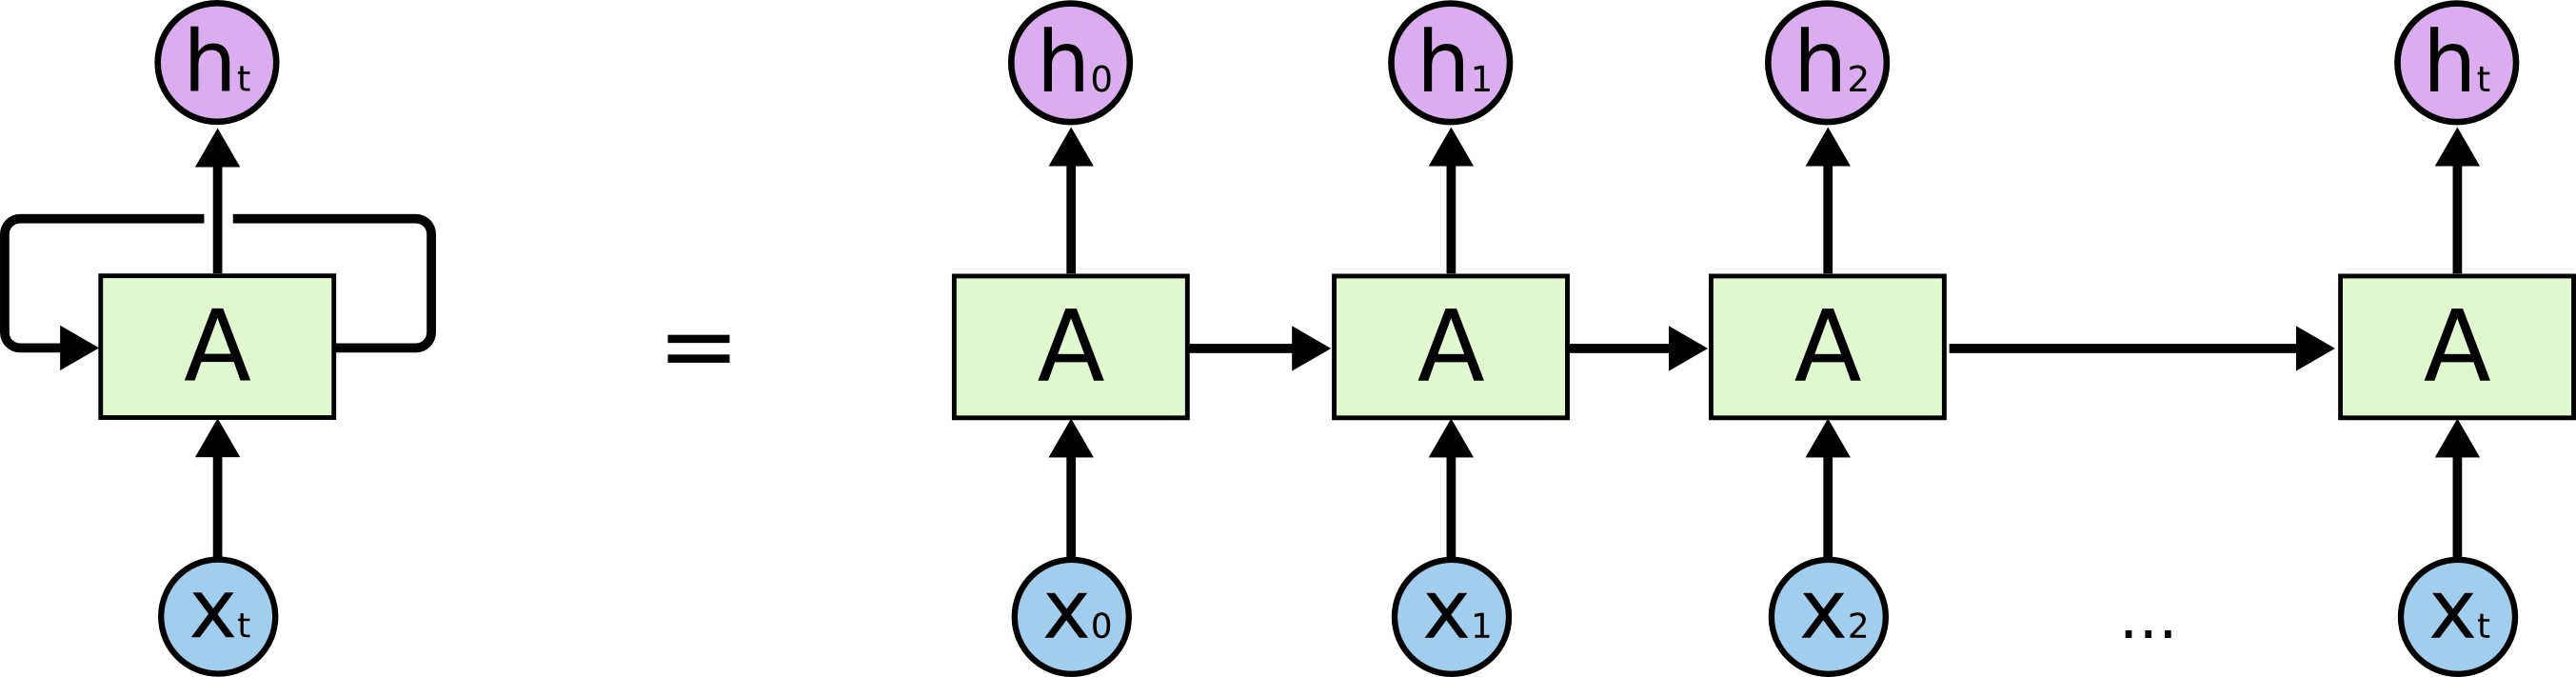
\includegraphics[width=\figureBigSize]
    {figure/model/RNN-unrolled.png}}
    \caption{\label{fig:rnn-unrolled} Recurrent Neural Network đã được trải ra.}
\end{figure}

Bản chất giống như chuỗi này cho thấy các Recurrent neural network có liên quan mật thiết đến các chuỗi và danh sách.
Nó sử dụng kiến trúc tự nhiên của mạng neuron để sử dụng cho dữ liệu đó.

Và chúng chắc chắn được sử dụng!
Trong vài năm qua, đã có những thành công đáng kinh ngạc khi áp dụng RNN cho nhiều vấn đề khác nhau: nhận dạng giọng
nói, mô hình ngôn ngữ, dịch thuật, chú thích hình ảnh.

Điều cần thiết cho những thành công này là việc sử dụng "LSTM", một loại Recurrent neural network rất đặc biệt, hoạt
động, cho nhiều tác vụ, tốt hơn nhiều so với phiên bản tiêu chuẩn. Hầu như tất cả các kết quả thú vị dựa trên các mạng thần kinh tái phát đều đạt được với chúng. Nó có những LSTM mà bài tiểu luận này sẽ khám phá.

\textbf{Vấn đề phụ thuộc xa} \\[0.2em]
Một trong những lời kêu gọi của RNN là ý tưởng rằng họ có thể kết nối thông tin trước đó với tác vụ hiện tại, chẳng
hạn như sử dụng các khung video trước đó có thể thông báo cho sự hiểu biết về khung hiện tại. Nếu RNN có thể làm điều
này, thì họ cực kỳ hữu ích. Nhưng họ có thể? Không hẳn.

Đôi khi, chúng ta chỉ cần nhìn vào thông tin gần đây để thực hiện nhiệm vụ hiện tại. Ví dụ, hãy xem xét một mô hình
ngôn ngữ đang cố gắng dự đoán từ tiếp theo dựa trên các từ trước đó. Nếu chúng ta đang cố gắng dự đoán từ cuối cùng
trong "các đám mây trên \textit{bầu trời}", thì chúng ta không cần bất kỳ bối cảnh nào nữa - đó là một điều khá rõ ràng,
từ tiếp theo sẽ là  \textit{bầu trời}. Trong những trường hợp như vậy, khi khoảng cách giữa thông tin liên quan và
địa điểm mà nó cần là nhỏ, RNN có thể học cách sử dụng thông tin trong quá khứ.

\begin{figure}[!htb]
    \center{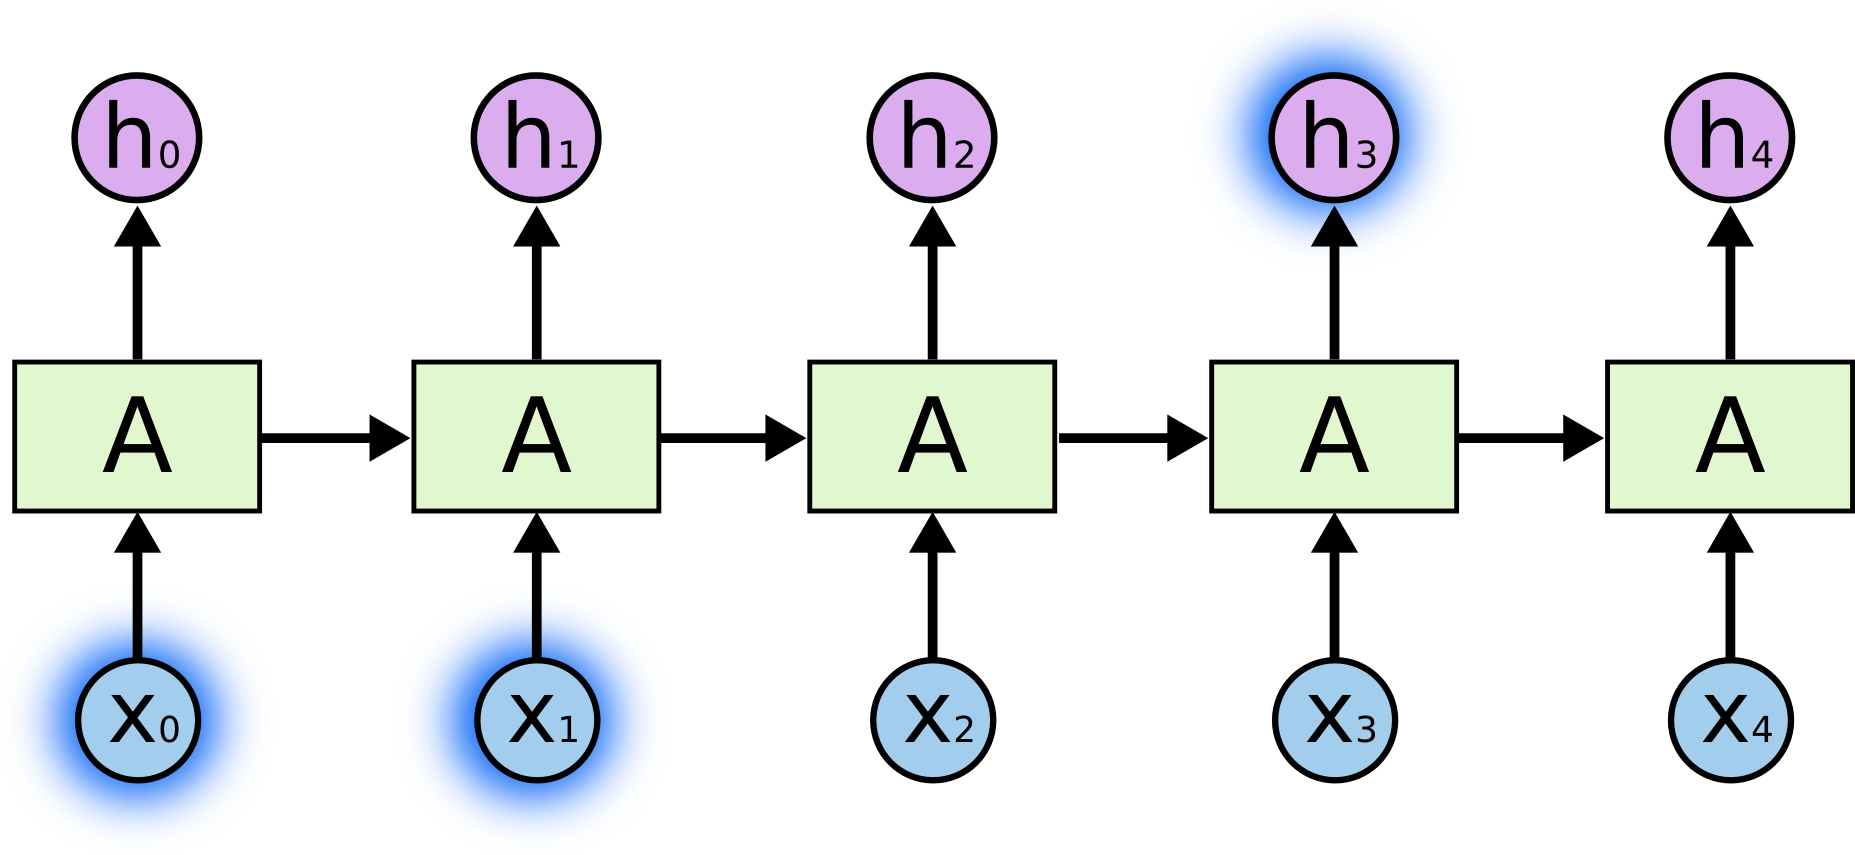
\includegraphics[width=\figureBigSize]
    {figure/model/RNN-shorttermdepdencies.png}}
\end{figure}

Nhưng cũng có những trường hợp chúng ta cần nhiều bối cảnh hơn. Cân nhắc việc cố gắng dự đoán từ cuối cùng trong văn
bản. "Tôi lớn lên ở Việt Nam. Tôi nói tiếng trôi chảy tiếng \textit{Việt}". Thông tin gần đây cho thấy từ tiếp theo có
lẽ là tên của một ngôn ngữ, nhưng nếu chúng ta muốn thu hẹp ngôn ngữ nào, chúng ta cần thu hẹp ngôn ngữ nào bối cảnh
của Việt Nam, từ phía trước. Nó hoàn toàn có thể cho khoảng cách giữa thông tin liên quan và điểm cần thiết để trở
nên rất lớn.

Thật không may, khi khoảng cách đó tăng lên, các RNN trở nên không thể học cách kết nối thông tin.
\begin{figure}[!htb]
    \center{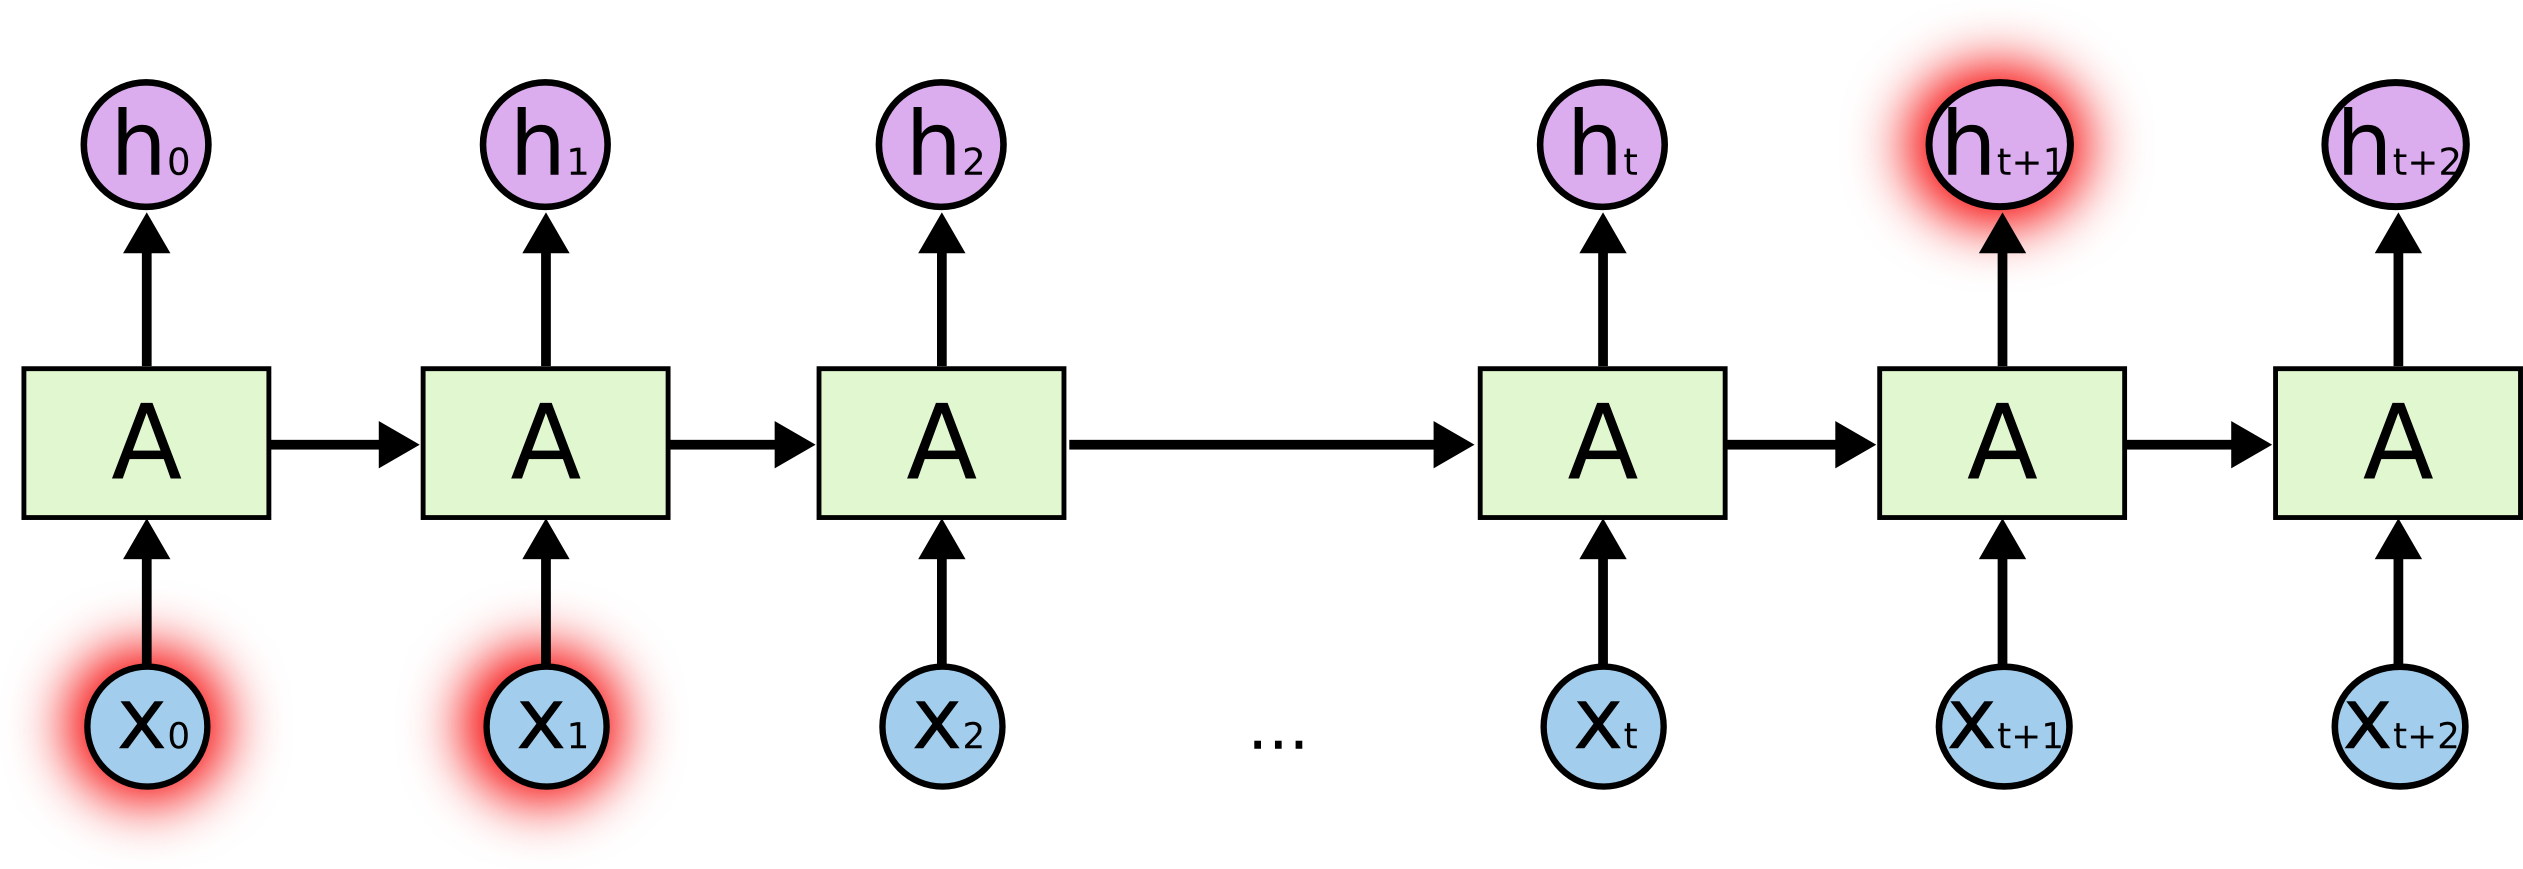
\includegraphics[width=\figureBigSize]
    {figure/model/RNN-longtermdependencies.png}}
\end{figure}


Về lý thuyết, các RNN hoàn toàn có khả năng xử lý các phụ thuộc dài hạn như vậy. Một người có thể cẩn thận chọn các
tham số cho họ để giải quyết các vấn đề về đồ chơi theo hình thức này. Đáng buồn thay, trong thực tế, RNNs don lồng
dường như có thể học chúng. Vấn đề đã được khám phá sâu bởi Hochreiter (1991) [German] và Bengio, et al. (1994),
người đã tìm thấy một số lý do khá cơ bản tại sao nó có thể khó khăn.

Rất may, LSTMs không có vấn đề này!

\textbf{Mạng LSTM} \\[0.2em]

Long Short Term Memory (mạng bộ nhớ dài ngắn hạn) - thường được gọi là LSTM của - - là một loại RNN đặc biệt, có khả
năng học các phụ thuộc xa. Chúng được giới thiệu bởi Hochreiter & Schmidhuber (1997), và được nhiều người tinh
chỉnh và phổ biến. Chúng hoạt động rất tốt trong nhiều vấn đề lớn, và hiện đang được sử dụng rộng rãi.

Các LSTM được thiết kế rõ ràng để tránh vấn đề phụ thuộc dài hạn. Ghi nhớ thông tin trong thời gian dài thực tế là
hành vi mặc định của nó, không phải là thứ khó khăn để học!

Tất cả các mạng thần kinh tái phát có dạng một chuỗi các module lặp lại của mạng thần kinh. Trong các RNN tiêu chuẩn,
module lặp lại này sẽ có cấu trúc rất đơn giản, chẳng hạn như một lớp \(tanh\) duy nhất.

\begin{figure}[!htb]
    \center{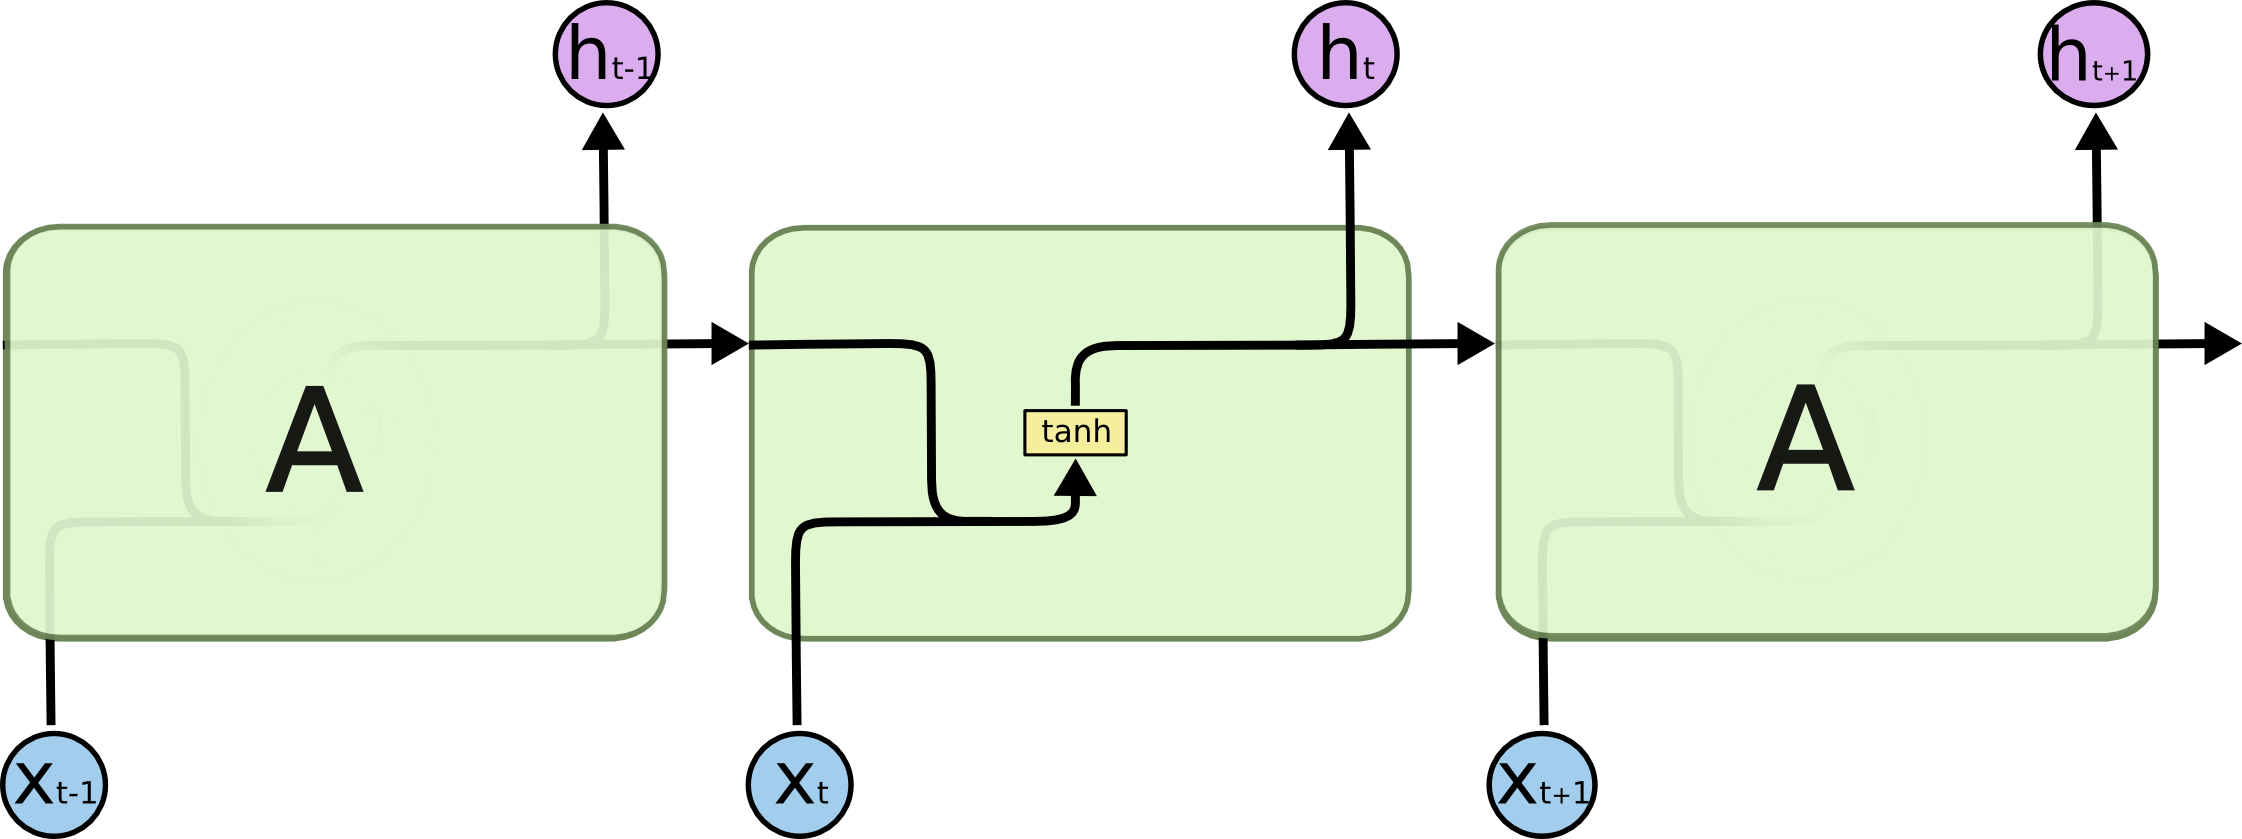
\includegraphics[width=\figureBigSize]
    {figure/model/LSTM3-SimpleRNN.png}}
    \caption{\label{fig:lstm3-simpleRNN} Module lặp trong RNN chuẩn chứa một lớp duy nhất.}
\end{figure}

LSTMs cũng có cấu trúc chuỗi, nhưng các module lặp có một cấu trúc khác. Thay vì có một lớp
mạng thần kinh duy nhất,nó có bốn lớp, tương tác theo một cách rất đặc biệt.

\begin{figure}[!htb]
    \center{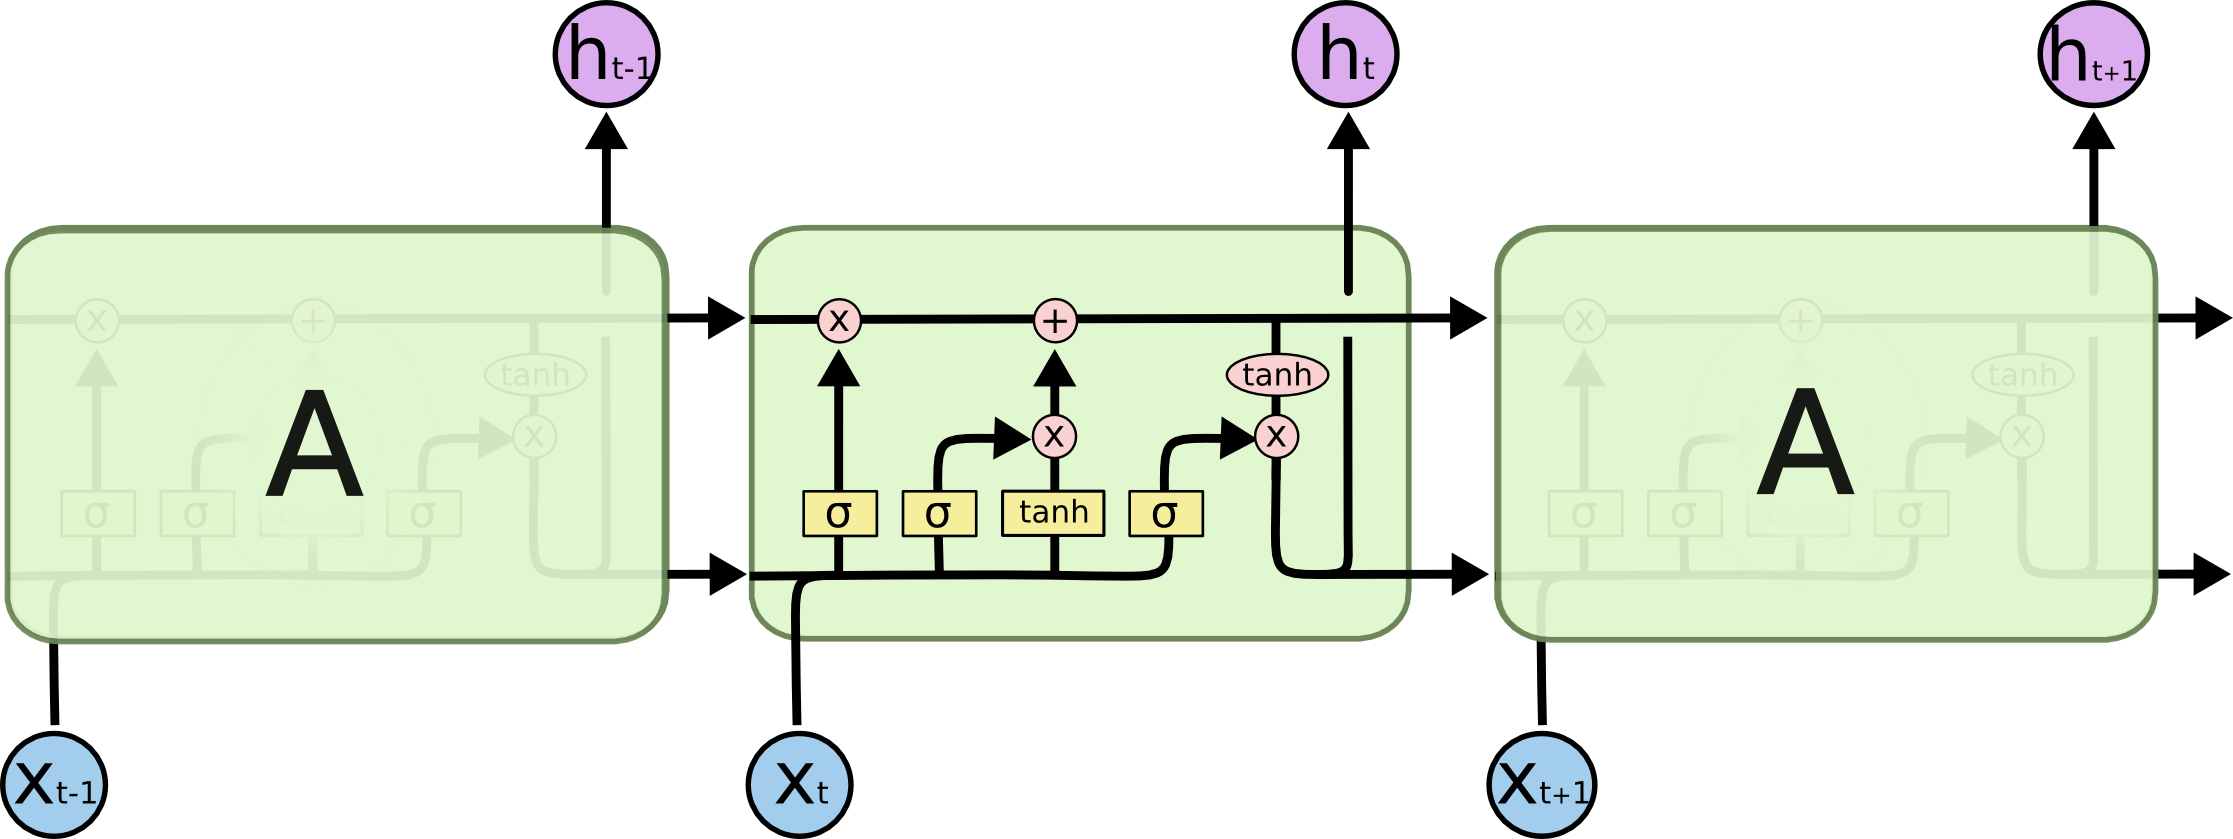
\includegraphics[width=\figureBigSize]
    {figure/model/LSTM3-chain.png}}
    \caption{\label{fig:lstm3-chain} Module lặp trong LSTM chứa 4 lớp tương tác.}
\end{figure}

\begin{figure}[!htb]
    \center{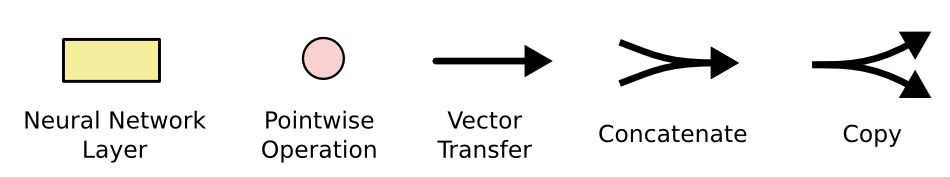
\includegraphics[width=\figureBigSize]
    {figure/model/LSTM2-notation.png}}
    \caption{\label{fig:lstm2-notation} Các ký hiệu trong LSTM.}
\end{figure}

Trong sơ đồ trên, mỗi dòng mang toàn bộ một vector, từ đầu ra của một nút đến đầu vào của các nút khác. Các vòng tròn
màu hồng đại diện cho các phép toán, như phép cộng vector, trong khi các hình chữ nhật màu vàng biểu thị các mạng
thần kinh để học. Các dòng hợp nhất biểu thị việc ghép nối, trong khi một dòng phân tách biểu thị nội dung của nó được
sao chép và các bản sao đi đến các vị trí khác nhau.

\textbf{Ý tưởng chính của LSTM} \\[0.2em]

Ý tưởng chính của LSTM là ô trạng thái, đường ngang chạy qua đỉnh sơ đồ.

Dòng trạng thái giống như một băng chuyền. Nó chạy thẳng xuống toàn bộ chuỗi, chỉ với một số tương tác tuyến tính nhỏ
dọc bên cạnh, dễ dàng cho thông tin truyền theo.

\begin{figure}[!htb]
    \center{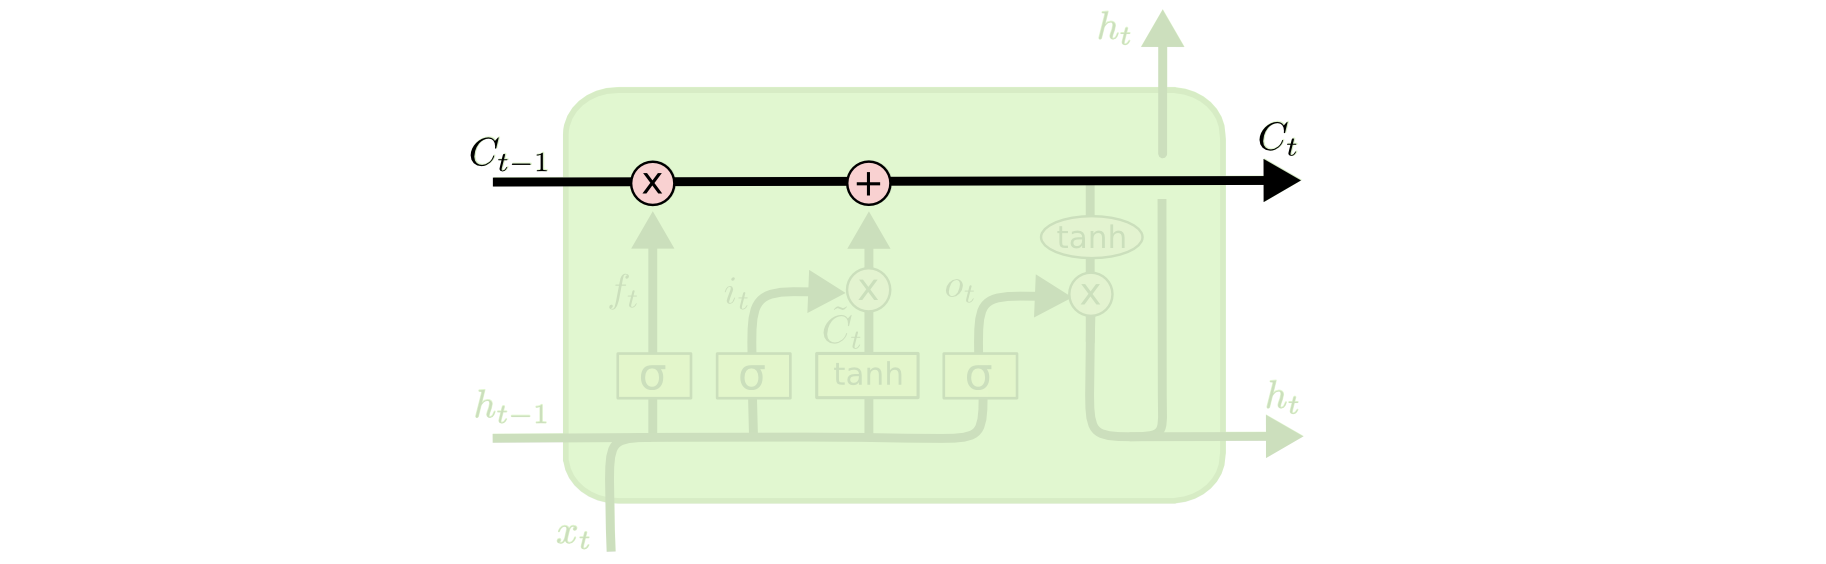
\includegraphics[width=\figureBigSize]
    {figure/model/LSTM3-C-line.png}}
\end{figure}

LSTM có khả năng loại bỏ hoặc thêm thông tin vào ô trạng thái, được điều chỉnh cẩn thận bởi các cấu trúc gọi là
cổng.

Cổng là một cấu trúc điều khiển thông tin thông qua. Chúng được cấu tạo từ một lớp lưới thần kinh \(sigmold\) và
một phép toán nhân.

\begin{figure}[!htb]
    \center{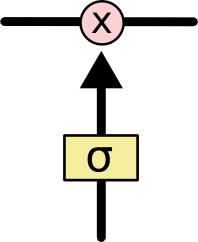
\includegraphics[width=1cm]
    {figure/model/LSTM3-gate.png}}
\end{figure}

Đầu ra của các lớp \(sigmoid\) có giá trị \([0, 1]\), mô tả mức độ cho qua. Giá
trị bằng \(0\) có nghĩa là không để bất cứ thứ gì qua, trong khi giá trị của \(1\) nghĩa
là có thể cho phép mọi thứ thông qua!

Một LSTM có ba trong cổng này, để bảo vệ và kiểm soát trạng thái tế bào.

\textbf{Các bước LSTM hoạt động} \\[0.2em]

Bước đầu tiên trong LSTM  là quyết định thông tin nào đi ra khỏi ô trạng thái. Quyết định này được đưa ra bởi
một lớp sigmoid được gọi là lớp "cổng quên". Nó dựa vào giá trị của \(h_{t-1}\) và \(x_t\), và đưa ra một số từ 0
đến 1 tương ứng với mỗi số ô trạng thái \(c_{t-1}\). Số 1 có nghĩa là giữ lại toàn bộ thông tin trong khi đó số 0 nghĩa
là hãy quên nó đi.

Hãy xem ví dụ của chúng ta về một mô hình ngôn ngữ đang cố gắng dự đoán từ tiếp theo dựa trên tất cả các từ trước đó.
Trong một vấn đề như vậy, ô trạng thái có thể bao gồm vai vế của ngữ hiện tại, để có thể sử dụng các đại từ nhân xưng
một cách chính xác. Khi có một chủ ngữ mới, nó sẽ quên đi vai vế của chủ ngữ cũ.

\begin{figure}[!htb]
    \center{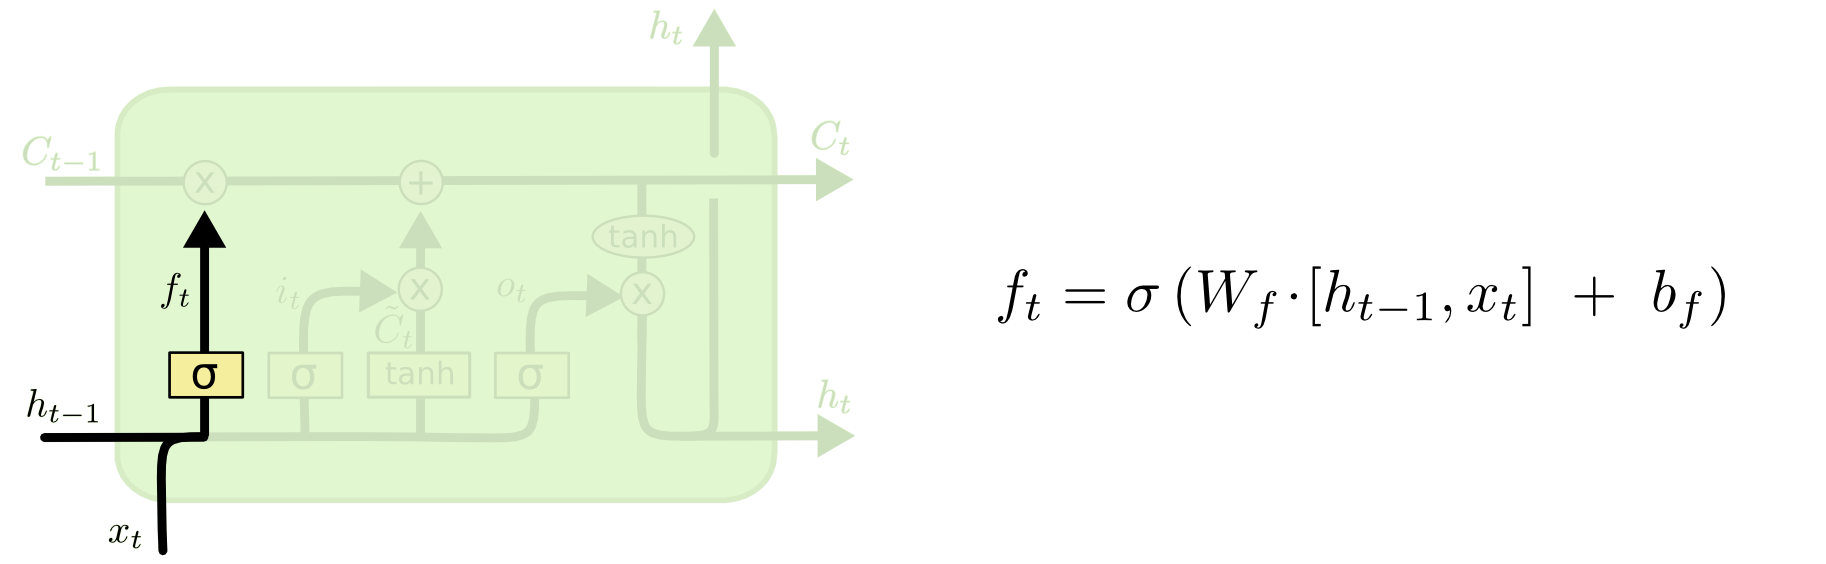
\includegraphics[width=\figureBigSize]
    {figure/model/LSTM3-focus-f.png}}
\end{figure}

Bước tiếp theo là quyết định những thông tin mới sẽ lưu trữ trong ô trạng thái. Việc này có hai phần. Đầu tiên,
một lớp sigmoid được gọi là lớp "cổng đầu vào" quyết định giá trị nào sẽ cập nhật. Tiếp theo, một lớp \(tanh\)
tạo ra một vector các giá trị ứng cử viên mới, \(C_t\), có thể được thêm vào ô trạng thái. Sau đó sẽ kết hợp  cả hai
để tạo ra một bản cập nhật cho trạng thái.

Trong ví dụ về mô hình ngôn ngữ, chúng tôi muốn thêm vai vế của chủ ngữ mới vào ô trạng thái, để thay thế chủ ngữ đã
quên.
\begin{figure}[!htb]
    \center{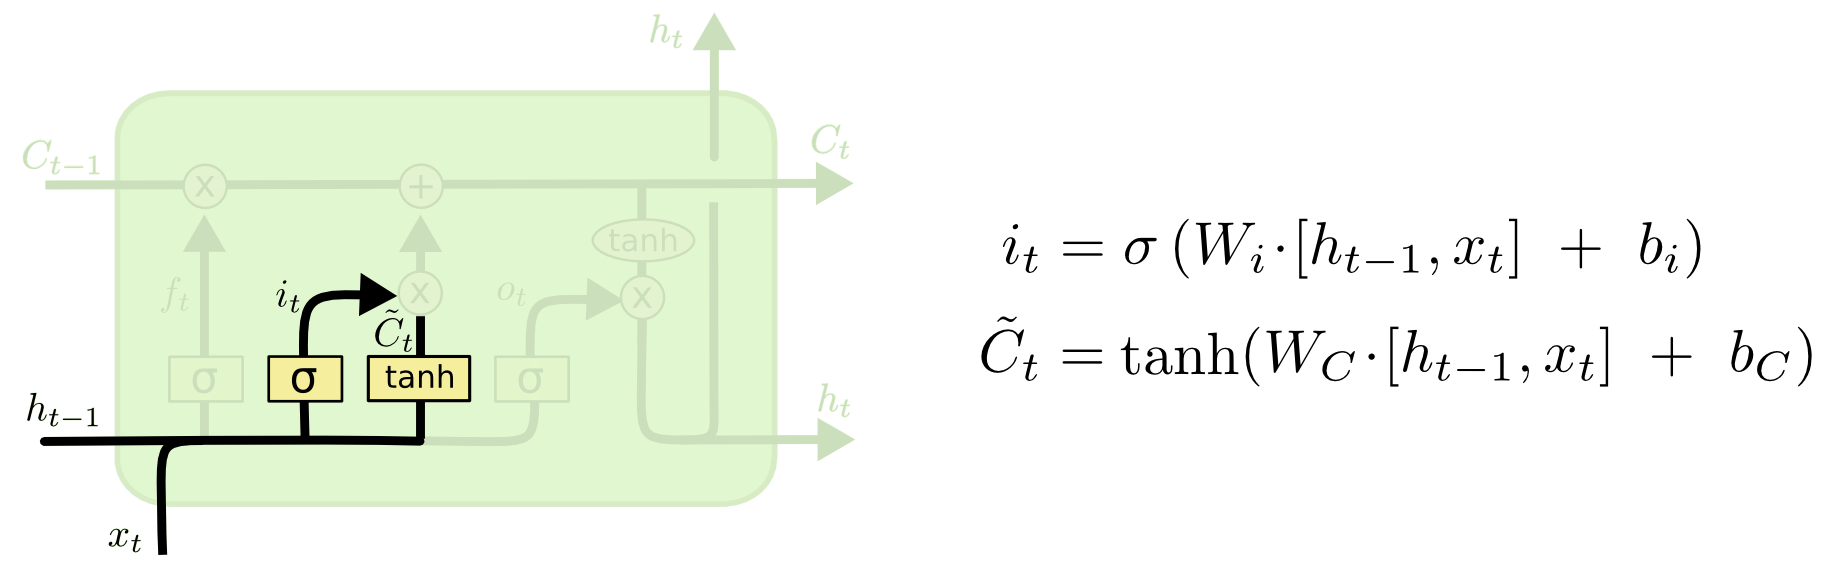
\includegraphics[width=\figureBigSize]
    {figure/model/LSTM3-focus-i.png}}
\end{figure}

Bây giờ, sẽ cập nhật ô trạng thái cũ, \(C_{t-1}\), sang ô trạng thái mới \(C_{t}\). Các bước trước đã quyết định phải
quên và nhớ những gì, giờ là lúc thực hiện nó.

Nhân ô trạng thái vũ với \(f_t\), quên đi những điều quyết định quên trước đó. Sau đó, cộng với \
i_t*\widetilde{C}_t\).
Đây là giá trị ứng viên mới, được tính theo mức độ cập nhật từng giá trị trạng thái.

Trong trường hợp của mô hình ngôn ngữ, đây là lúc thực sự bỏ thông tin về vai về và thêm thông tin mới, như đã quyết định trong các bước trước.
\begin{figure}[!htb]
    \center{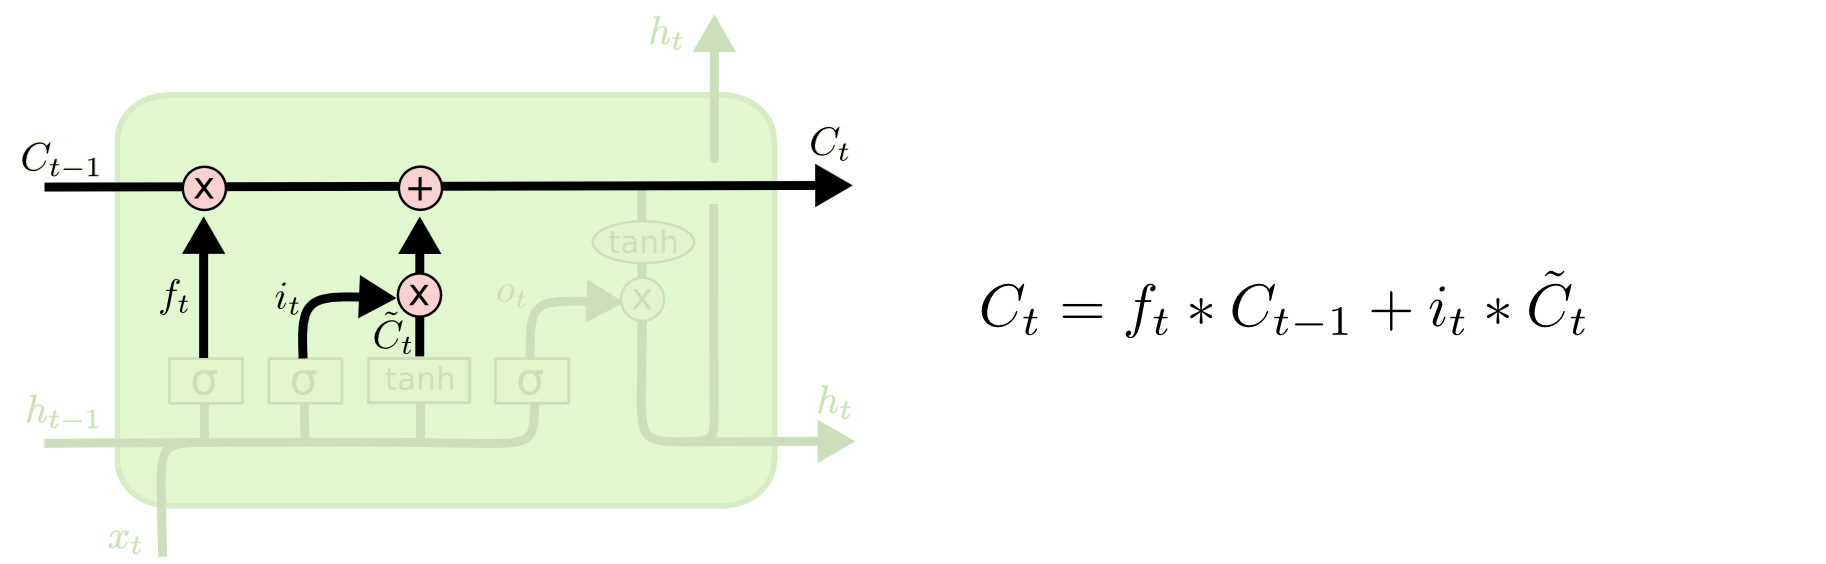
\includegraphics[width=\figureBigSize]
    {figure/model/LSTM3-focus-C.png}}
\end{figure}
Cuối cùng là quyết định những gì sẽ xuất ra. Đầu ra sẽ được lọc dựa vào ô trạng thái. Đầu tiên, chạy một lớp
\(sigmoid\) quyết định phần nào của ô trạng thái mà sẽ xuất ra. Sau đó, đưa ô trạng thái qua hàm
\(tanh\) (để đẩy các giá trị nằm trong khoảng -1 đến 1) và nhân nó với đầu ra của cổng \(sigmoid\), do đó chỉ đưa ra
các dữ liệu đã quyết định

Đối với ví dụ về mô hình ngôn ngữ, vì nó chỉ nhìn thấy một chủ ngữ, nó có thể muốn đưa ra thông tin có liên quan đến
một động từ, trong trường hợp đó là những gì sắp diễn ra. Ví dụ, nó có thể xuất ra vai vế của chủ ngữ , để biết được
cách dùng từ với chủ ngữ đó.

\section{Seq2seq}
\label{sec:model:seq2seq}
Lê Viết Quốc khiến bạn không khỏi bất ngờ khi anh chính là một nhân vật quan trọng trong lĩnh vực trí tuệ nhân tạo tại Google. Quốc được biết đến với "Google Brain".
Vào năm 2014, Quốc đề xuất trình tự chuỗi (Seq2seq) học với nhà nghiên cứu Google Ilya Sutskever và Oriol Vinyals. Nó là một khung công cụ - một thư viện các mã lệnh (framework) giải mã bộ mã hóa có mục đích đào tạo các mô hình để chuyển đổi các chuỗi từ một tên miền này sang miền khác, chẳng hạn như chuyển đổi các câu sang các ngôn ngữ khác nhau.
Seq2seq learning đòi hỏi ít sự lựa chọn trong thiết kế kỹ thuật hơn và cho phép hệ thống dịch của Google hoạt động hiệu quả và chính xác trên các tệp dữ liệu khổng lồ. Nó chủ yếu được sử dụng cho các hệ thống dịch máy và được chứng minh là có thể ứng dụng được ở nhiều mảng hơn, bao gồm tóm tắt văn bản, các cuộc hội thoại với trí tuệ nhân tạo, và trả lời câu hỏi.

Sau đó, Quốc tiếp tục phát minh ra Doc2vec – một thuật toán không giám sát sử dụng cho việc hiển thị các nội dung có độ dài cố định từ các đoạn văn bản có độ dài biến đổi, chẳng hạn như câu, đoạn văn và các tài liệu.
Doc2vec là phần mở rộng của Word2vec, được giới thiệu vào năm 2013 bởi nghiên cứu sinh của Google, Tomas Mikolov. Ý tưởng của nó là mỗi từ có thể được biểu diễn bằng một vec-tơ, có thể được tự động học từ một tập hợp văn bản. Quốc sử dụng vector cho các đoạn văn để mô hình có thể tạo ra sự hiển thị - trình chiếu của tài liệu, bất chấp độ dài của nó.
Những nỗ lực nghiên cứu của Quốc đã được đền đáp. Trong năm 2016, Google đã công bố hệ thống dịch máy Nơ-ron (Neural Machine Translation System), sử dụng trí tuệ nhân tạo AI để tạo ra các bản dịch tốt hơn và tự nhiên hơn.
\textbf{Các ứng dụng của Seq2seq} \\[0.2em]
Một chuỗi để mô hình trình tự nằm đằng sau nhiều hệ thống mà bạn phải đối mặt trên cơ sở hàng ngày. Chẳng hạn, mô hình seq2seq hỗ trợ các ứng dụng như Google Dịch, thiết bị hỗ trợ giọng nói và chatbot trực tuyến. Nói chung, các ứng dụng này bao gồm:

Dịch máy - một bài báo năm 2016 của Google cho thấy cách tiếp cận chất lượng dịch thuật mô hình seq2seq hoặc vượt qua tất cả các kết quả được công bố hiện tại.

Nhận dạng giọng nói - một bài báo khác của Google so sánh các mô hình seq2seq hiện có về nhiệm vụ nhận dạng giọng nói.

Chú thích video - một bài báo năm 2015 cho thấy một seq2seq mang lại kết quả tuyệt vời như thế nào khi tạo mô tả phim.

Đây chỉ là một số ứng dụng mà seq2seq được xem là giải pháp tốt nhất. Mô hình này có thể được sử dụng như một giải pháp cho bất kỳ vấn đề dựa trên trình tự nào, đặc biệt là các vấn đề trong đó đầu vào và đầu ra có kích thước và danh mục khác nhau. Chúng ta sẽ nói nhiều hơn về cấu trúc mô hình dưới đây
 % INCLUDE: concepts
    % !TEX root = ../chatbot-report.tex
%
\chapter{Kết quả đạt được}
\label{sec:conclusion} % INCLUDE: conclusion
    \cleardoublepage

    % --------------------------
    % Back matter
    % --------------------------
    {%
    \setstretch{1.1}
    \renewcommand{\bibfont}{\normalfont\small}
    \setlength{\biblabelsep}{0pt}
    \setlength{\bibitemsep}{0.5\baselineskip plus 0.5\baselineskip}
    \printbibliography[nottype=online]
    \printbibliography[heading=subbibliography,title={Webseiten},type=online,prefixnumbers={@}]
    }
    \cleardoublepage

    \listoffigures
    \cleardoublepage

    \listoftables
    \cleardoublepage

    % !TEX root = ../thesis-example.tex
%
\pagestyle{empty}
\hfill
\vfill
\pdfbookmark[0]{Colophon}{Colophon}
\section*{Colophon}

This thesis was typeset with \LaTeXe.
It uses the \textit{Clean Thesis} style developed by Ricardo Langner.
The design of the \textit{Clean Thesis} style is inspired by user guide documents from Apple Inc.

Download the \textit{Clean Thesis} style at \url{http://cleanthesis.der-ric.de/}.

    \cleardoublepage

    % !TEX root = ../chatbot-report.tex
%
%************************************************
% Declaration
%************************************************
\pdfbookmark[0]{Declaration}{Declaration}
\chapter*{Declaration}
\label{sec:declaration}
\thispagestyle{empty}

You can put your declaration here, to declare that you have completed your work solely and only with the help of the references you mentioned.

\bigskip

\noindent\textit{\thesisUniversityCity, \thesisDate}

\smallskip

\begin{flushright}
	\begin{minipage}{5cm}
		\rule{\textwidth}{1pt}
		\centering\thesisName
	\end{minipage}
\end{flushright}

%*****************************************
%*****************************************

    \clearpage
    \newpage
    \mbox{}

    % **************************************************
    % End of Document CONTENT
    % **************************************************
\end{document}
